% Shared editable artwork for all v1-v4 arrangements.
\documentclass[tikz,border=0pt]{standalone}
\usepackage{fontspec}
\setsansfont{Arial}
\setmainfont{Arial}
\usepackage{graphicx,amsmath,pgfplots}
\pgfplotsset{compat=1.18}
\usetikzlibrary{arrows.meta,calc}

% Matplotlib colours in workflow order: C0, C1, C2, C8, C4.
\definecolor{C0}{HTML}{1F77B4}
\definecolor{C1}{HTML}{FF7F0E}
\definecolor{C2}{HTML}{2CA02C}
\definecolor{C8}{HTML}{BCBD22}
\definecolor{C4}{HTML}{9467BD}
\definecolor{labelInk}{HTML}{002A48}
\colorlet{simInk}{C0!72!black}
\colorlet{crystalInk}{C1!70!black}
\colorlet{cztInk}{C8!60!black}

\tikzset{
  focusing/.style={x=1cm,y=1cm,line cap=round,line join=round,
    every node/.style={font=\sffamily,text=labelInk,inner sep=0pt}},
  title/.style={font=\sffamily\bfseries\fontsize{12}{14}\selectfont},
  detail/.style={font=\sffamily\fontsize{9}{11}\selectfont,align=center},
  project/.style={font=\sffamily\bfseries\fontsize{29}{31}\selectfont},
  badge/.style={draw=black,line width=.32mm},
  flow/.style={draw=black!85,line width=.42mm,
    -{Stealth[length=2.3mm,width=1.7mm]},shorten <=11.6mm,shorten >=11.6mm},
  axisArrow/.style={black,line width=.20mm,-{Stealth[length=1.0mm,width=.8mm]}},
  mathlabel/.style={font=\fontsize{8}{9}\selectfont}
}

% Original XAS/XANES paths and lettering; only the badge/accent colours change.
\newcommand{\DrawXAS}[1]{%
  \node at (#1) {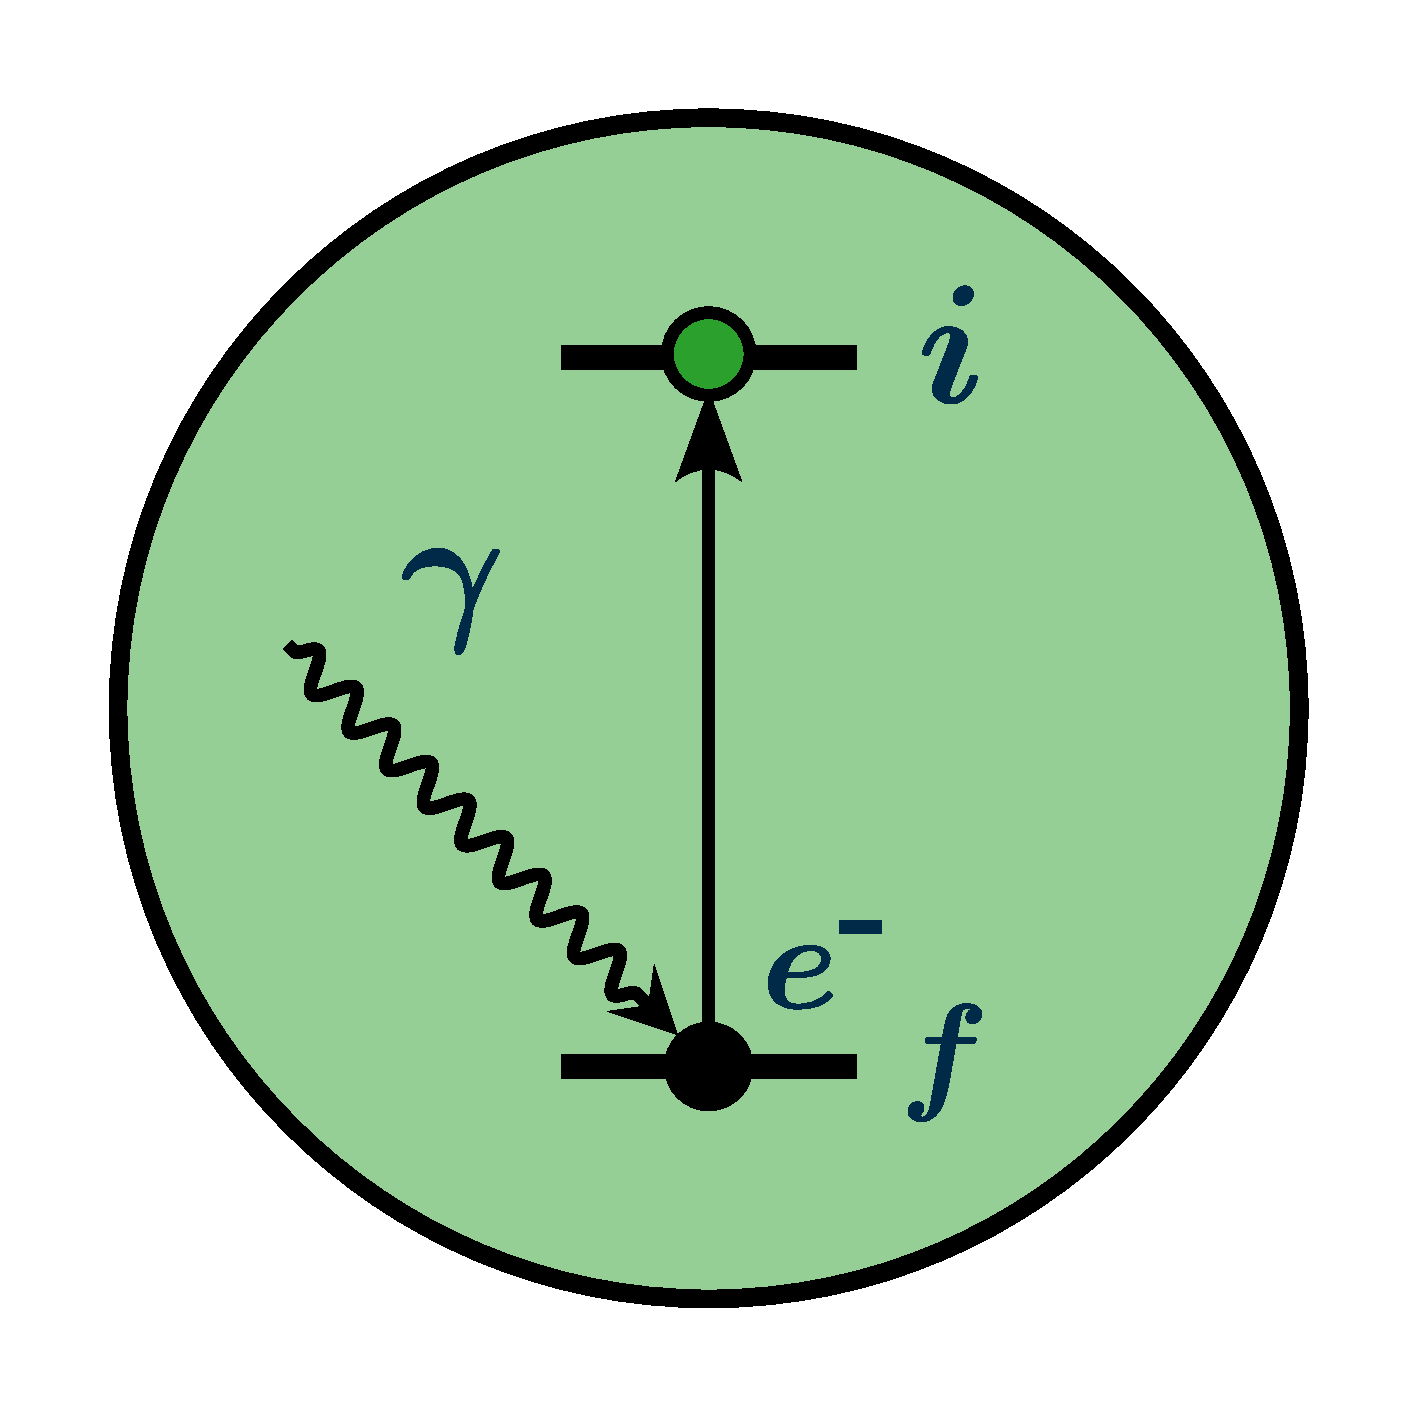
\includegraphics[width=21.6mm,
    trim=18mm 18mm 18mm 18mm,clip]{.build/XAS_C2.pdf}};
}
\newcommand{\DrawXANES}[1]{%
  \node at (#1) {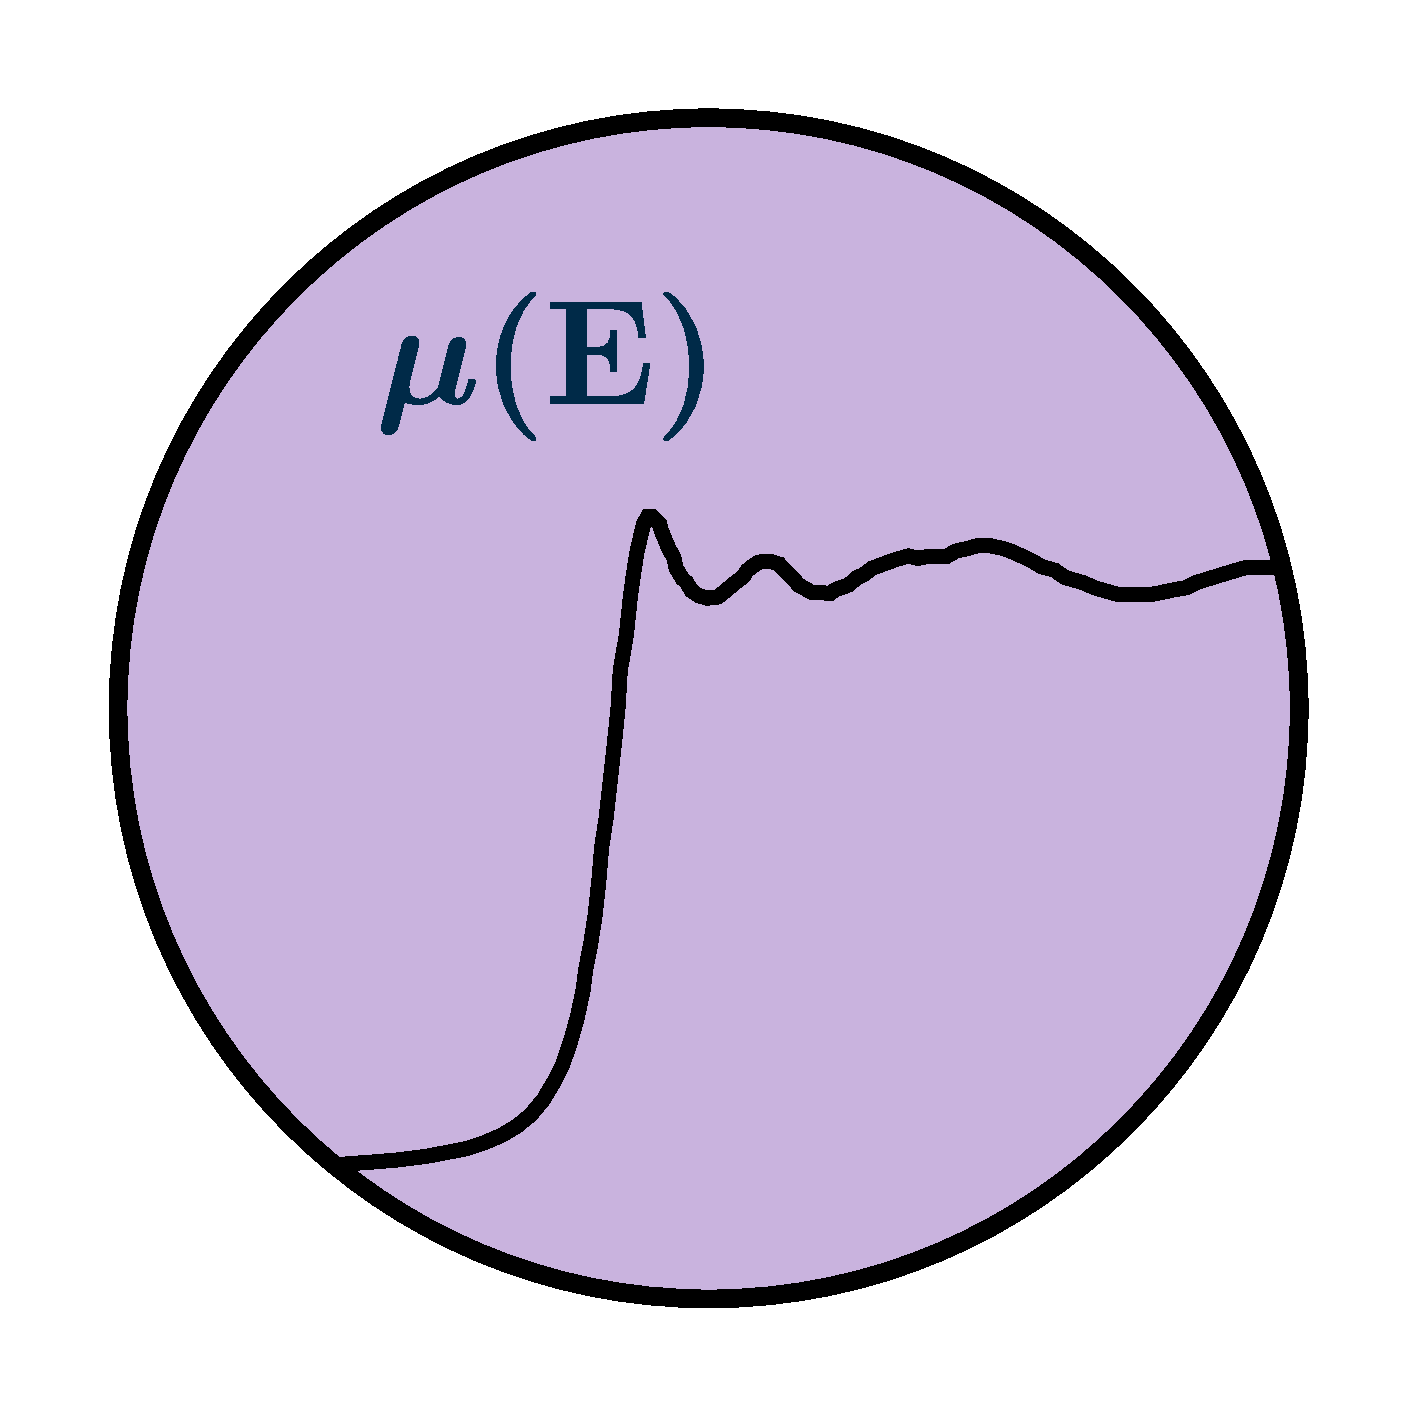
\includegraphics[width=21.6mm,
    trim=18mm 18mm 18mm 18mm,clip]{.build/XANES_C4.pdf}};
}

% Ray tracing above; a sampled detector-response distribution below.
% The ray bundle and histogram are schematic, not calculated performance.
\newcommand{\DrawSimulation}[1]{%
\begin{scope}[shift={(#1)}]
  \filldraw[badge,fill=C0!50!white] (0,0) circle (1.06);
  % Separate rays make the source -> optic -> detector path readable.
  \foreach \xx/\yy in {-.25/.60,0/.63,.25/.60}{
    \draw[simInk,line width=.24mm]
      (-.72,.16) -- (\xx,\yy) -- (.72,.16);
  }
  \draw[simInk,line width=.27mm,-{Stealth[length=1.15mm,width=.9mm]}]
    (-.54,.2775) -- (-.30,.4342);
  \draw[simInk,line width=.27mm,-{Stealth[length=1.15mm,width=.9mm]}]
    (.30,.4342) -- (.54,.2775);
  % A source aperture, shallow optic, and a segmented detector.
  \filldraw[fill=simInk,draw=black,line width=.23mm,rounded corners=.4mm]
    (-.87,-.005) rectangle (-.69,.325);
  \filldraw[fill=C0!20!white,draw=black,line width=.14mm]
    (-.69,.16) circle (.045);
  % Concave face points down, towards the incident and reflected rays.
  \path[fill=C0,draw=black,line width=.25mm]
    (-.36,.69) .. controls (-.12,.77) and (.12,.77) .. (.36,.69)
    -- (.36,.57) .. controls (.12,.65) and (-.12,.65) .. (-.36,.57) -- cycle;
  \filldraw[fill=simInk,draw=black,line width=.23mm]
    (.70,-.04) rectangle (.87,.35);
  \foreach \yy in {.035,.13,.225}{
    \fill[C0!20!white] (.735,\yy) rectangle ++(.10,.055);
  }
  % Monte Carlo-style bins plus a smooth response envelope.
  \foreach \xx/\hh in {-.57/.025,-.45/.075,-.33/.19,-.21/.34,-.09/.43,.03/.35,.15/.21,.27/.08,.39/.025}{
    \filldraw[fill=C0,draw=simInk,line width=.12mm]
      (\xx,-.70) rectangle ++(.105,\hh);
  }
  \draw[black,line width=.26mm]
    (-.64,-.69) .. controls (-.42,-.69) and (-.35,-.61) .. (-.25,-.42)
    .. controls (-.13,-.15) and (.02,-.15) .. (.14,-.43)
    .. controls (.23,-.62) and (.33,-.69) .. (.57,-.69);
  \draw[axisArrow] (-.73,-.73) -- (.74,-.73);
  \draw[axisArrow] (-.73,-.73) -- (-.73,-.22);
\end{scope}
}

% Flat perfect Ge(220) sigma reflectivity at 10 keV; see README for provenance.
% The smooth shallow wafer is symbolic and carries no atomic lattice grid.
\newcommand{\DrawCrystal}[1]{%
\begin{scope}[shift={(#1)}]
  \filldraw[badge,fill=C1!50!white] (0,0) circle (1.06);
  \begin{axis}[at={(-.64cm,.13cm)},anchor=south west,
    width=1.28cm,height=.52cm,scale only axis,
    xmin=-100,xmax=100,ymin=0,ymax=1.05,hide axis]
    \addplot[draw=crystalInk,line width=.31mm]
      table[x index=0,y index=1] {4_Crystal/reflectivity_Ge220.dat};
  \end{axis}
  \draw[axisArrow] (-.67,.11) -- (.72,.11);
  \draw[axisArrow] (-.67,.11) -- (-.67,.67);
  \node[mathlabel] at (-.48,.65) {$\mathcal{R}$};
  \node[mathlabel] at (.56,-.055) {$\Delta\theta$};
  \path[fill=crystalInk,draw=black,line width=.25mm]
    (-.72,-.34) .. controls (-.25,-.44) and (.25,-.44) .. (.72,-.34)
    -- (.72,-.50) .. controls (.25,-.60) and (-.25,-.60) .. (-.72,-.50) -- cycle;
  \path[fill=C1,draw=black,line width=.25mm]
    (-.72,-.18) .. controls (-.25,-.28) and (.25,-.28) .. (.72,-.18)
    -- (.72,-.34) .. controls (.25,-.44) and (-.25,-.44) .. (-.72,-.34) -- cycle;
  \node[font=\sffamily\bfseries\fontsize{8}{9}\selectfont] at (0,-.79) {Ge};
\end{scope}
}

% A schematic 20-channel sensor and the original, unmodified waveform samples.
% Black curves; the two classification symbols use the circle's darker C8.
% Only the last 34% of the displayed time window is cropped; data are untouched.
\newcommand{\DrawCZT}[1]{%
\begin{scope}[shift={(#1)}]
  \filldraw[badge,fill=C8!50!white] (0,0) circle (1.06);
  \path[fill=cztInk,draw=black,line width=.20mm]
    (-.79,.51) -- (.71,.51) -- (.80,.61) -- (.80,.39)
    -- (.71,.29) -- (-.79,.29) -- cycle;
  \path[fill=C8,draw=black,line width=.20mm]
    (-.79,.51) -- (.71,.51) -- (.80,.61) -- (-.70,.61) -- cycle;
  \draw[black,line width=.16mm] (.71,.51) -- (.71,.29);
  \foreach \i in {0,...,19}{
    \pgfmathsetmacro{\xx}{-.747+.073*\i}
    \filldraw[fill=C8!15!white,draw=cztInk,line width=.09mm]
      (\xx,.35) rectangle ++(.043,.105);
  }
  \begin{axis}[at={(-.65cm,-.66cm)},anchor=south west,
    width=1.39cm,height=.85cm,scale only axis,
    xmin=0,xmax=1,ymin=-1.15,ymax=1.15,hide axis,
    restrict x to domain=0:.66,unbounded coords=discard,filter discard warning=false]
    \addplot[black,line width=.29mm]
      table[x index=0,y index=1] {5_Pulse_Shape/waveforms.dat};
    \addplot[black,line width=.29mm]
      table[x index=0,y expr=\thisrowno{2}-1.12] {5_Pulse_Shape/waveforms.dat};
  \end{axis}
  \draw[cztInk,line width=.38mm] (.36,.04) -- (.44,-.04) -- (.58,.16);
  \draw[cztInk,line width=.38mm] (.38,-.38) -- (.54,-.54) (.38,-.54) -- (.54,-.38);
\end{scope}
}
